\documentclass[10pt,a4paper]{article}
\usepackage[utf8]{inputenc}
\usepackage[english]{babel}
\usepackage{csquotes}
\usepackage{amsmath}
\usepackage{amsfonts}
\usepackage{amssymb}
\usepackage{graphicx}
\usepackage[margin=0.5in]{geometry}
\usepackage{amsthm}
\usepackage{enumitem}
\usepackage{tikz}
\usetikzlibrary{calc}
\newtheorem{question}{Question}
\newtheorem*{question*}{Question}
\newtheorem{theorem}{Theorem}
\newtheorem*{theorem*}{Theorem}
\newtheorem{lemma}{Lemma}

\theoremstyle{definition}
\newtheorem{answer}{Answer}
\newtheorem*{answer*}{Answer}


\title{Complex Analysis Homework 4}
\author{Colin Williams}

\begin{document}
\maketitle

\section*{Question 2}

Plot the image $\gamma^*$ of the curve $\gamma$ in the following cases, indicating how the image is traced:
\begin{enumerate}[label = (\alph*)]
\item $\gamma(t) = 1 + ie^{it}, t\in [0, \pi]$
\item $\gamma$ is the join of three line segments: $[-1, 1], [1,1+i]$, and $[1+i, -1-i]$
\end{enumerate}

\begin{answer*}{\textbf{(a)}}
\\First, note that the curve $e^{it}, t \in [0,\pi]$ simply has an image of the upper semi-circle centered at 0 going counter-clockwise. Next, note that multiplying any $a + bi \in \mathbb{C}$ by $i$ gives $-b + ai$ which is a $90^{\circ}$ rotation counter-clockwise. Thus, the curve $ie^{it}, t \in [0, \pi]$ would have the image of the left semi-circle centered at 0 going counter-clockwise. Lastly, adding 1 simply shifts the center of the semi-circle right 1 unit, so $\gamma(t) = 1 + ie^{it}, t \in [0,\pi]$ have the image $\gamma^*$ represented as the following:

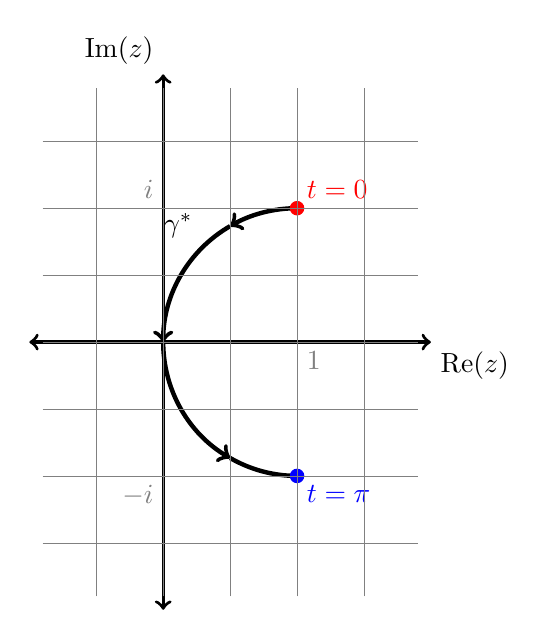
\begin{tikzpicture}[scale = 1.7]
\draw [very thick, <->] (-1,0) -- (2,0);
\node [below right] at (2,0) {Re$(z)$};
\draw [very thick, <->] (0,-2) -- (0,2);
\node [above left] at (0,2) {Im$(z)$};
\draw [black, ultra thick, ->] (1,1) arc (90: 120: 1);
\draw [black, ultra thick, ->] (1/2,{sqrt(3)/2}) arc (120: 180: 1);
\draw [black, ultra thick, ->] (0,0) arc (180: 240: 1);
\draw [black, ultra thick] (1/2,{-sqrt(3)/2}) arc (240: 270: 1);
\node [above left] at ({-1/sqrt(2) + 1},{1/sqrt(2)}) {$\gamma^*$};
\draw[fill, red] (1,1) circle [radius=0.05];
\node [above right, red] at (1,1) {$t = 0$};
\draw[fill, blue] (1,-1) circle [radius=0.05];
\node [below right, blue] at (1,-1) {$t = \pi$};
\draw[step=0.5,gray, ultra thin] (-0.9,-1.9) grid (1.9,1.9);
\node [below right, gray] at (1,0) {1};
\node [above left, gray] at (0,1) {$i$};
\node [below left, gray] at (0,-1) {$-i$};
\end{tikzpicture}

\end{answer*}

\begin{answer*}{\textbf{(b)}}
\\The way that $\gamma$ is defined, it should consist of line segments going to the following points in this order: $-1, 1, 1 + i, -1-i$. Thus, $\gamma^*$ looks like the following:

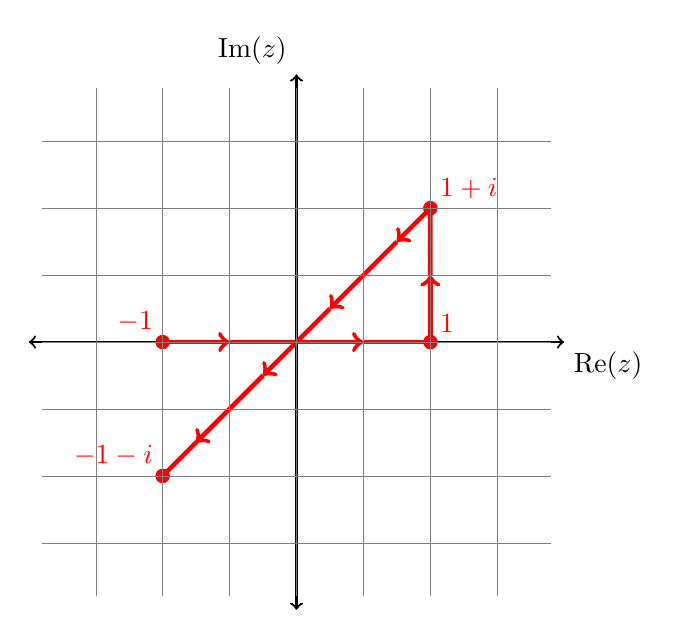
\begin{tikzpicture}[scale = 1.7]
\draw [thick, <->] (-2,0) -- (2,0);
\node [below right] at (2,0) {Re$(z)$};
\draw [thick, <->] (0,-2) -- (0,2);
\node [above left] at (0,2) {Im$(z)$};

\draw [ultra thick, ->, red] (-1,0) -- (-.5,0);
\draw [ultra thick, ->, red] (-.5,0) -- (.5, 0);
\draw [ultra thick, ->, red] (.5,0) -- (1,0) -- (1, .5);
\draw [ultra thick, ->, red] (1,.5) -- (1,1) -- (.75,.75);
\draw [ultra thick, ->, red] (.75,.75) -- (.25,.25);
\draw [ultra thick, ->, red] (.25,.25) -- (-.25,-.25);
\draw [ultra thick, ->, red] (-.25,-.25) -- (-.75,-.75);
\draw [ultra thick, red] (-.25,-.25) -- (-1,-1);

\draw[fill, red] (-1,0) circle [radius=0.05];
\node [above left, red] at (-1,0) {$-1$};
\draw[fill, red] (1,0) circle [radius=0.05];
\node [above right, red] at (1,0) {$1$};
\draw[fill, red] (1,1) circle [radius=0.05];
\node [above right, red] at (1,1) {$1 + i$};
\draw[fill, red] (-1,-1) circle [radius=0.05];
\node [above left, red] at (-1,-1) {$-1 -i$};

\draw[step=0.5,gray, ultra thin] (-1.9,-1.9) grid (1.9,1.9);
\end{tikzpicture}

\end{answer*}

\end{document}